% ============================================================================
% IEEE Transactions on Transportation Electrification
% LLMBO-MO: LLM-Augmented Multiobjective Bayesian Optimization
% for Battery Fast-Charging Protocol Design
% ============================================================================
\documentclass[journal]{IEEEtran}
\usepackage[utf8]{inputenc}
\usepackage[T1]{fontenc}
\usepackage{cite}
\usepackage{amsmath,amssymb,amsfonts}
\usepackage{algorithm}
\usepackage{algpseudocode}
\usepackage{graphicx}
\usepackage{microtype}
\usepackage{tikz}
\usetikzlibrary{arrows.meta,backgrounds,calc,fit,positioning,shapes.geometric}
\usepackage{textcomp}
\usepackage{xcolor}
\usepackage{booktabs}
\usepackage{multirow}
\usepackage{array}
\usepackage{url}
\usepackage[hidelinks,bookmarksnumbered]{hyperref}
\urlstyle{same}
\renewcommand{\figureautorefname}{Figure}
\renewcommand{\tableautorefname}{Table}

\graphicspath{{figures/}}
\hyphenation{op-tical net-works semi-conduc-tor}

\newcommand{\btheta}{\boldsymbol{\theta}}
\newcommand{\bw}{\boldsymbol{w}}
\newcommand{\bD}{\mathcal{D}}
\newcommand{\bS}{\mathcal{S}}
\newcommand{\bL}{\mathcal{L}}
\newcommand{\bW}{\mathcal{W}}
\newcommand{\bP}{\mathcal{P}}
\newcommand{\bG}{\mathcal{G}}
\newcommand{\R}{\mathbb{R}}

% Canonical manuscript-facing values.
% Main Chen2020 and Ecker2015 comparisons are reported over five matched trials.

% Chen2020 main comparison: final HV (mean +/- sample SD).
\newcommand{\ChenLLMBOMean}{0.3848}
\newcommand{\ChenLLMBOStd}{0.0073}
\newcommand{\ChenParEGOMean}{0.3520}
\newcommand{\ChenParEGOStd}{0.0169}
\newcommand{\ChenFinalGain}{9.3\%}

\newcommand{\ChenNSGAMean}{0.3265}
\newcommand{\ChenNSGAStd}{0.0220}
\newcommand{\ChenNSGAGain}{17.9\%}
\newcommand{\ChenDISKMean}{0.3085}
\newcommand{\ChenDISKStd}{0.0267}
\newcommand{\ChenDISKGain}{24.8\%}
\newcommand{\ChenPIMDMean}{0.2941}
\newcommand{\ChenPIMDStd}{0.0195}
\newcommand{\ChenPIMDGain}{30.8\%}

% Ecker2015 main comparison.
\newcommand{\EckerParEGOMean}{0.4760}
\newcommand{\EckerParEGOStd}{0.0039}
\newcommand{\EckerLLMBOMean}{0.5605}
\newcommand{\EckerLLMBOStd}{0.0008}
\newcommand{\EckerMidParEGO}{0.4333}
\newcommand{\EckerMidLLMBO}{0.5559}
\newcommand{\EckerMidGain}{28.3\%}
\newcommand{\EckerFinalGain}{17.8\%}

% Objective-preprocessing diagnostic.
\newcommand{\NormMinMaxMean}{0.4146}
\newcommand{\NormMinMaxStd}{0.0067}
\newcommand{\NormZScoreMean}{0.4122}
\newcommand{\NormZScoreStd}{0.0078}
\newcommand{\NormNoneMean}{0.3826}
\newcommand{\NormNoneStd}{0.0358}
\newcommand{\NormMidMinMax}{0.3355}
\newcommand{\NormMidZScore}{0.3920}
\newcommand{\NormMidNone}{0.3255}

\newcommand{\OptimalLLMBOFinal}{49.4}
\newcommand{\OptimalParEGOFinal}{45.8}

% Chen2020 initialization study: ten matched trials.
\newcommand{\PromptHVGain}{0.05828}

% Short-budget Chen2020 component ablation:
% three matched trials, 6 initialization evaluations + 10 BO iterations.
\newcommand{\AblationTotalCalls}{16}
\newcommand{\AblationBaselineMean}{0.2907}
\newcommand{\AblationBaselineStd}{0.0451}
\newcommand{\AblationWarmMean}{0.3462}
\newcommand{\AblationWarmStd}{0.0109}
\newcommand{\AblationRegionMean}{0.2980}
\newcommand{\AblationRegionStd}{0.0462}
\newcommand{\AblationFullMean}{0.3500}
\newcommand{\AblationFullStd}{0.0039}
\newcommand{\AblationWarmGain}{+0.0555}
\newcommand{\AblationRegionGain}{+0.0072}
\newcommand{\AblationFullGain}{+0.0593}

% LLM-informed initialization portfolio hyperparameters.
% The weights balance the LLM heuristic score, the soft terminal-span
% penalty, the monotonicity indicator, and the decision-space diversity.
\newcommand{\OmegaPenalty}{0.20}
\newcommand{\OmegaMonotone}{0.10}
\newcommand{\OmegaDiversity}{0.30}
\newcommand{\SoftDeltaSK}{0.10}
\newcommand{\SoftWidth}{0.10}
% Augmented Tchebycheff and objective-scale hyperparameters.
\newcommand{\RhoAug}{0.05}
\newcommand{\RhoR}{0.30}


\begin{document}

\title{LLMBO-MO: Large Language Model-Augmented Multiobjective Bayesian Optimization\\
for Battery Fast-Charging Protocol Design}

\author{Anonymous~Authors%
}

\markboth{Submitted to IEEE Transactions on Transportation Electrification}%
{Anonymous Authors: LLMBO-MO for Battery Fast-Charging}

\maketitle
% ============================================================================
% Abstract (humanizer-informed revision; original narrative retained)
% ============================================================================
\begin{abstract}
Lithium-ion batteries are widely used in electric vehicles and energy-storage
systems, making efficient and reliable fast charging increasingly important.
As charging requirements become more diverse, charging strategies must balance
charging speed, safety, and battery degradation under different user
preferences. Bayesian optimization (BO) reduces the number of simulator
evaluations by using a probabilistic surrogate model and an acquisition
function to select candidate protocols. However, two challenges remain when
observations are scarce. First, uninformed initialization does not use available
battery-domain knowledge when selecting initial charging protocols. Second,
incorporating such knowledge during sequential BO requires accounting for the
changing trade-offs in multiobjective optimization. Large language models
(LLMs) offer a way to incorporate task-specific prior knowledge into BO.
Accordingly, this paper proposes LLMBO-MO, an LLM-guided multiobjective
Bayesian optimization framework for lithium-ion battery charging design.
LLMBO-MO first uses an LLM to propose initial charging protocols from
battery-domain knowledge, followed by candidate screening and diversity-aware
selection. During the early search, the LLM also proposes a preferred region
for the current scalarization weights. Region-Lift uses Gaussian process (GP)
posterior cross-covariance to apply bounded adjustments to the mean used in
expected improvement. These adjustments alter the ranking of candidate
protocols. Under a budget of 56 simulator evaluations, LLMBO-MO achieves a
9.3\% higher mean final hypervolume than ParEGO on Chen2020. An advantage over
ParEGO is also observed on Ecker2015.
\end{abstract}

\begin{IEEEkeywords}
Lithium-ion batteries, battery charging, Bayesian optimization,
large language models, multiobjective optimization.
\end{IEEEkeywords}

\IEEEpeerreviewmaketitle

% ============================================================================
% Section I: Introduction (humanizer-informed revision; original structure retained)
% ============================================================================

\section{Introduction}
\label{sec:introduction}

The growing use of lithium-ion batteries in electric vehicles and energy-storage
systems has increased the demand for efficient fast charging. Fast charging
requires balancing charging speed against thermal stress and degradation. For a
prescribed amount of charge, shortening the charging time requires a higher
average current. However, high charging rates increase polarization and heat
generation and can promote degradation, with the response depending on
temperature and state of charge (SOC)~\cite{refFastChargeReview}.
Charging-protocol design therefore involves selecting how the current varies
across charging stages while reaching a target SOC within prescribed current,
voltage, and temperature limits. The competing objectives of charging time,
thermal response, and battery health motivate a constrained multiobjective
formulation that provides alternative protocols for different operating
preferences~\cite{nref2,refGPA}.

Evaluating these trade-offs is expensive. Physical charging and aging tests
consume cells and laboratory time; in particular, directly measuring cycle
life can require months of testing~\cite{nref3}. Battery models allow candidate
protocols to be assessed in simulation, reducing reliance on physical
experiments during the design stage. Nevertheless, electrochemical models
require repeated numerical solution of coupled transport and reaction
equations, often together with thermal and aging dynamics. Consequently,
replacing experiments with simulation reduces the cost of each evaluation but
does not eliminate the computational burden of searching across many
protocols~\cite{nref7,nref8}. This motivates sample-efficient optimization
methods that require fewer simulator evaluations.

Bayesian optimization (BO) addresses this evaluation cost through sequential
surrogate modeling and acquisition-based sampling. A probabilistic surrogate,
commonly a Gaussian process (GP), estimates both objective values and predictive
uncertainty from evaluated candidates. An acquisition function combines these
estimates to select the next candidate, allowing many alternatives to be
compared using the inexpensive surrogate before one is evaluated by the battery
simulator~\cite{nref6}.

Several studies have established the relevance of BO to fast charging.
Attia \emph{et al.} combined early cycle-life prediction with BO to optimize
fast-charging protocols experimentally, reducing both the duration and number
of tests~\cite{nref3}. Jiang \emph{et al.} investigated BO for minimum-time
charging subject to degradation-related constraints and compared acquisition
functions for multistage protocols~\cite{nref7}. Wang and Jiang extended this
approach to charging-time and cycle-life trade-offs using Tchebycheff
scalarization and constrained BO~\cite{nref8}. More recently,
Zhu \emph{et al.} combined early degradation prediction with multiobjective BO
to consider knee-point capacity and cycle life~\cite{refZhuMOBO}.
GP-assisted evolutionary charging design has also addressed multiple user
preferences while reducing simulation requirements~\cite{refGPA}. Despite
these advances, the search is driven primarily by numerical observations
collected during the optimization process.

Battery-domain knowledge can complement these numerical observations when only
a few evaluations are available. In particular, prior knowledge of how
charging stages affect thermal response and degradation can help identify
useful regions of the protocol space. Prior-guided BO has already been
investigated for battery charging: Jeong \emph{et al.} incorporated a simplified
aging model to guide the search for health-conscious
protocols~\cite{refPriorCharging}. Such model-based prior information, however,
requires an explicit quantitative representation of the available knowledge.
Qualitative knowledge concerning charging-variable meanings, operating
practices, and objective trade-offs is more difficult to incorporate directly
into BO, particularly when candidate selection must account for multiple
competing objectives.

Large language models (LLMs) can interpret such descriptions and generate
candidate suggestions conditioned on the optimization context. Liu \emph{et al.}
introduced LLAMBO and investigated LLM-based warm starting, surrogate modeling,
and candidate sampling, with empirical results on hyperparameter
optimization~\cite{nref12}. In the battery domain, Kuai \emph{et al.} applied
LLM-enhanced BO to electrochemical parameter identification~\cite{refKuaiLLMBO}.
These studies suggest that LLMs can provide task-specific prior information when
numerical observations are scarce. For multiobjective charging design, however,
the guidance must also reflect the trade-off currently being optimized.

These observations suggest two points at which LLM-derived knowledge may be
useful under a limited simulation budget. First, it can improve the initial
design by proposing plausible charging protocols while maintaining sufficient
diversity. Second, it can provide regional guidance during sequential BO
according to the current objective trade-off. Because the scalarization weights
change across iterations, a region that is suitable for one objective trade-off
may be less suitable for another.

This paper proposes \emph{LLM-guided Multiobjective Bayesian Optimization
(LLMBO-MO)} for multistage battery charging. The method combines LLM-informed
initialization with covariance-based regional guidance in a decomposition-based
BO framework. The regional-guidance component is inspired by the region-lifted
preference mechanism of LGBO~\cite{ref5} and is adapted here to the
weight-conditioned multiobjective setting. We refer to this adaptation as
Region-Lift. The main contributions are as follows:

\begin{itemize}

    \item We develop an LLM-informed initialization strategy that uses
    charging-variable definitions, operating constraints, and battery-domain
    knowledge to propose initial protocols. Candidate screening and
    diversity-aware selection are combined with random valid protocols to
    construct the initial simulation design.

    \item We adapt region-lifted preference guidance to decomposition-based
    multiobjective BO by conditioning the regional preference on the active
    scalarization weight and restricting its influence to the early search
    stage. GP posterior cross-covariance translates the regional preference
    into an adjustment of the mean used to compute expected improvement (EI).
    Standard EI is used when no valid regional preference is available.

    \item We evaluate LLMBO-MO on the Chen2020 and Ecker2015 battery
    parameterizations under limited simulation budgets. LLMBO-MO achieves a
    higher final mean hypervolume than ParEGO on both parameterizations at the
    tested budget. Initialization and ablation studies show that
    battery-specific initialization accounts for most of the improvement in
    the short-budget experiments.

\end{itemize}

The remainder of this paper is organized as follows.
Sections~\ref{sec:problem} and~\ref{sec:model_section} present the charging
problem and battery model, respectively. Section~\ref{sec:method} describes
LLMBO-MO. Section~\ref{sec:experiments} reports the experiments, and
Section~\ref{sec:conclusion} concludes the paper.

\section{Problem Formulation}
\label{sec:problem}

We consider multistage constant-current (MCC) charging from an initial SOC to
a prescribed target. Each protocol is evaluated by its charging time, peak
temperature rise, and charging-induced degradation. Figure~\ref{fig:charging_problem}
summarizes the decision variables, objectives, and constraints.

\begin{figure}[!t]
\centering
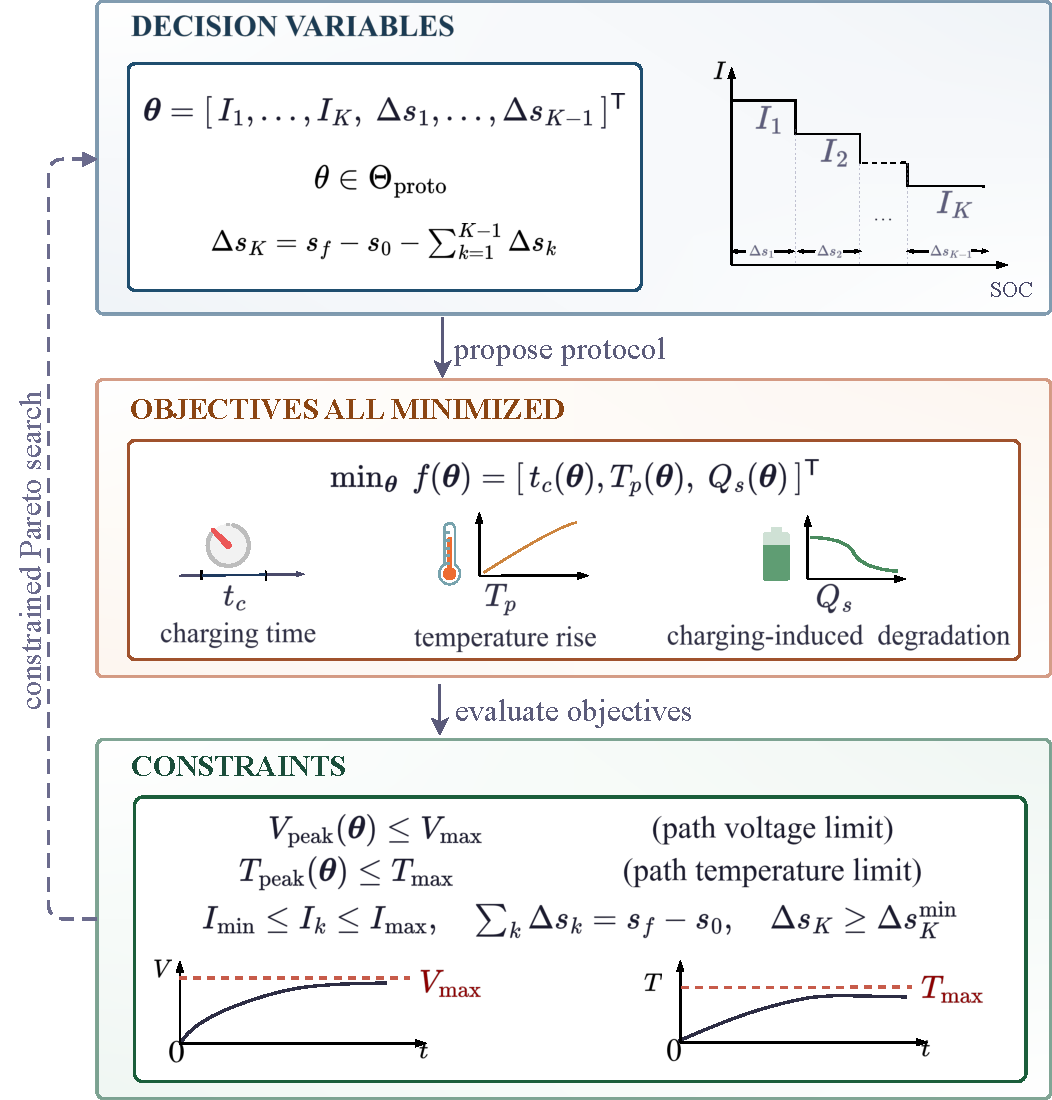
\includegraphics[width=\columnwidth]{fig1.pdf}
\caption{Fast-charging multiobjective design problem.}
\label{fig:charging_problem}
\end{figure}


\subsection{Multistage Constant-Current Protocol}

A $K$-stage protocol applies a current $I_k$ over an SOC increment $\Delta s_k$
at stage $k$. The initial and target SOCs are $s_0$ and $s_f$, respectively.
The independent decision variables are
\begin{equation}
\theta=[I_1,\ldots,I_K,\Delta s_1,\ldots,\Delta s_{K-1}]^\top
\label{eq:protocol}
\end{equation}
and the final SOC increment is
\begin{equation}
\Delta s_K=s_f-s_0-\sum_{k=1}^{K-1}\Delta s_k
\label{eq:terminal_soc}
\end{equation}
Each current and SOC increment is restricted to its prescribed interval. The
last increment must also exceed a positive lower bound so that every stage has
nonzero duration.
% AUTHOR_CHECK P1: Supply the actual current/SOC bounds, terminal lower bound,
% initial and target SOCs, and effective capacities from the experiment configs.

Following~\cite{nref7,nref8}, we optimize SOC increments rather than stage
durations. The current and charge delivered in each stage determine its
duration, giving the total charging time
\begin{equation}
t_c(\theta)=3600Q_{\mathrm{eff}}\sum_{k=1}^{K}\frac{\Delta s_k}{I_k}
\label{eq:charging_time}
\end{equation}
where $Q_{\mathrm{eff}}$ is the effective cell capacity in Ah and current is
measured in A. The experiments use $K=3$, giving five independent decision
variables.

\subsection{Constrained Multiobjective Charging Design}

The three objectives are minimized jointly:
\begin{equation}
\min_{\theta}\quad
\mathbf f(\theta)=[t_c(\theta),\,T_p(\theta),\,Q_s(\theta)]^\top
\label{eq:cmop}
\end{equation}
Here, $T_p$ is the peak temperature rise and $Q_s$ is the aging indicator
defined in Section~\ref{sec:model_section}. In addition to the bounds on the
decision variables, the charging trajectory must satisfy
\begin{equation}
U(t;\theta)\le U_{\max},\quad
T(t;\theta)\le T_{\max},\quad
0\le t\le t_c(\theta)
\label{eq:operating_constraints}
\end{equation}
where $U_{\max}$ and $T_{\max}$ are the voltage and temperature limits. A
protocol is infeasible if it violates either limit or fails to reach $s_f$;
such protocols are excluded from the Pareto archive.
% AUTHOR_CHECK P2: Exclusion from the Pareto archive does not specify how
% infeasible/failed simulations are represented in the GP or acquisition.

Higher charging currents reduce charging time but generally increase the
thermal and aging costs. We therefore seek a set of feasible nondominated
protocols, allowing the charging-time, temperature, and degradation trade-off
to be chosen for the operating requirement.

\section{Electrochemical--Thermal--Aging Model}
\label{sec:model_section}

\subsection{Electrochemical Model}
\label{sec:model}

The single particle model with electrolyte dynamics (SPMe) describes the
battery's electrochemical response~\cite{refSPMe}. It accounts for lithium
diffusion in representative solid particles of both electrodes and transport
through the electrolyte. This reduced model retains the electrochemical
dynamics needed for charging simulation at a lower computational cost than a
full porous-electrode model.

The terminal voltage is calculated as~\cite{refSPMe}
\begin{equation}
U=U_{\mathrm{eq}}+\eta_r+\eta_d+\Delta\Phi
\label{eq:voltage}
\end{equation}
where $U_{\mathrm{eq}}$ is the equilibrium potential, $\eta_r$ is the ohmic
overpotential, $\eta_d$ is the concentration overpotential, and $\Delta\Phi$
is the average potential difference in the electrolyte. SOC is obtained from
the solid-phase lithium concentration. The SPMe equations and their derivation
are given in~\cite{refSPMe}.
% AUTHOR_CHECK M1: Verify the voltage decomposition and the meanings/signs of
% eta_r, eta_d, and DeltaPhi against the model actually implemented.

\subsection{Thermal Model}

A lumped thermal model gives the cell temperature:
\begin{equation}
\rho_{\mathrm{eff}}\frac{\partial T}{\partial t}=\bar Q-\frac{hA}{V}(T-T_a)
\label{eq:thermal_balance}
\end{equation}
Here, $\rho_{\mathrm{eff}}$ is the effective volumetric heat capacity,
$\bar Q$ is the average volumetric heat-generation rate, $h$ is the
heat-transfer coefficient, $A$ is the heat-dissipation area, $V$ is the cell
volume, and $T_a$ is the ambient temperature. The effective heat capacity is
\begin{equation}
\rho_{\mathrm{eff}}=\frac{\sum_k\rho_kC_{p,k}L_k}{\sum_kL_k}
\label{eq:rho_eff}
\end{equation}
where $\rho_k$, $C_{p,k}$, and $L_k$ denote density, specific heat capacity,
and thickness. The sum includes the two current collectors, the two
electrodes, and the separator.

The thermal objective is the maximum temperature rise during charging:
\begin{equation}
T_p(\theta)=\max_{0\le t\le t_c(\theta)}[T(t)-T_0]
\label{eq:peak_temp}
\end{equation}
where $T_0$ is the initial cell temperature.

\subsection{Aging Model}
\label{sec:aging}

Charging-induced degradation is evaluated with the semi-empirical
capacity-loss model of Suri and Onori~\cite{refAgingModel}:
\begin{equation}
Q_s(\xi,Ah)=\sigma_{\mathrm{fun}}(\xi)Ah^z
\label{eq:aging}
\end{equation}
The vector $\xi=(\mathrm{SOC},I,T)$ contains the average SOC, current, and
temperature during charging; $Ah$ is the charge throughput; and $z$ is the
power-law exponent. The severity factor is
% AUTHOR_CHECK M2: The uploaded equation is preserved below. Its denominator
% uses 273.15+T, whereas the thermal settings use kelvin. Verify the conversion
% in the implementation before choosing a Celsius or kelvin notation here.
\begin{equation}
\sigma_{\mathrm{fun}}(\xi)=(\alpha\,\mathrm{SOC}+\beta)\exp\!\left(\frac{-E_a+\eta_a I}{R_{\mathrm{gas}}(273.15+T)}\right)
\label{eq:severity}
\end{equation}
where $\alpha$ and $\beta$ describe SOC dependence, $\eta_a$ describes current
dependence, $E_a$ is the activation energy, and $R_{\mathrm{gas}}$ is the
universal gas constant. We use $Q_s$ as a relative degradation indicator for
one charging process, rather than as a prediction of battery end-of-life.
% AUTHOR_CHECK M3: Supply the coefficients, averaging/aggregation rule, and
% justification for using this aging model with each battery parameterization.

% ============================================================================
% Section IV: Proposed LLMBO-MO
% Revised to emphasize the core methodological idea and reduce implementation-level detail.
% ============================================================================

\section{Proposed LLMBO-MO}
\label{sec:method}

\subsection{Framework}
\label{sec:framework}

LLMBO-MO uses battery-domain knowledge to guide the choice of protocols to
simulate. Figure~\ref{fig:framework} shows the optimization loop. The LLM
first proposes an initial set of protocols. During the early BO iterations,
it also suggests a region for the current trade-off among objectives. The BO
optimizer scalarizes the observed objectives, fits a GP, and selects the next
protocol by maximizing EI. Evaluating that protocol with the battery model
provides its objective values and feasibility, which are used to update the
data set $D$ and the feasible Pareto archive $P$. The loop stops when the
simulation budget is exhausted.

\begin{figure}[!t]
\centering
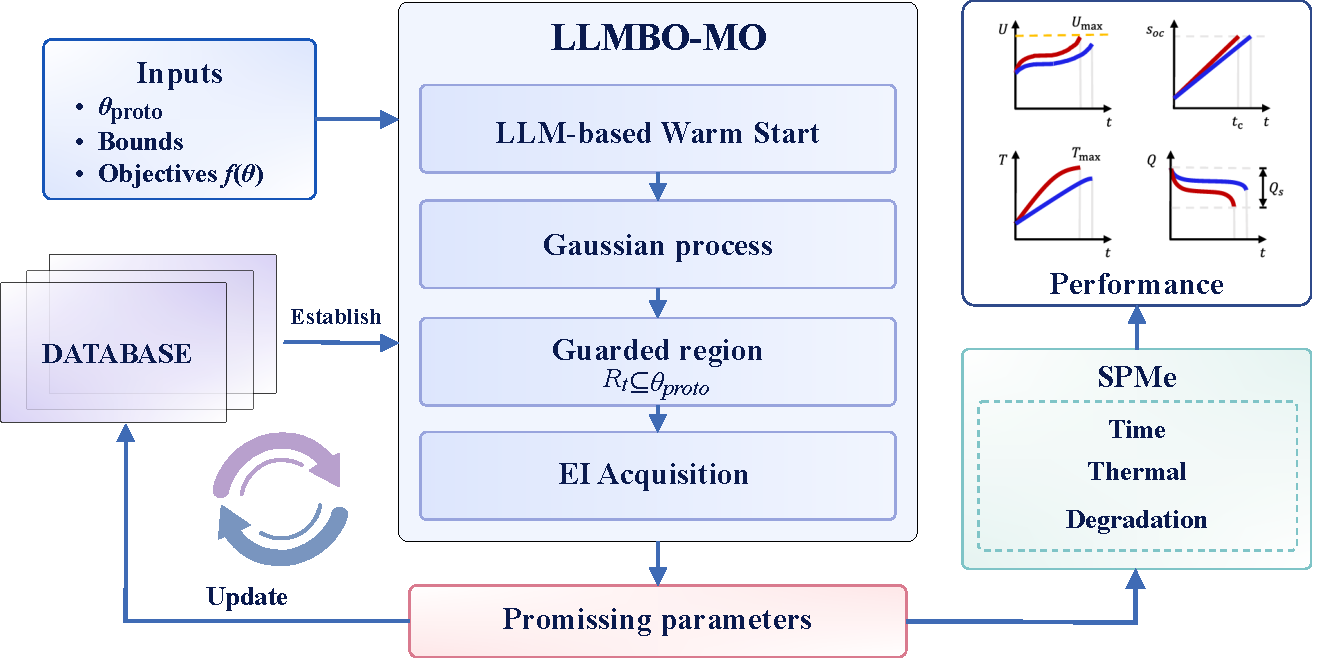
\includegraphics[width=\columnwidth]{fig2.pdf}
\caption{Structure of the proposed LLMBO-MO framework}
\label{fig:framework}
\end{figure}


\subsection{Decomposition-Based Multiobjective BO}
\label{sec:parego_backbone}

The numerical optimizer follows the decomposition-based approach of
ParEGO~\cite{ref4}. A set $W$ of nonnegative weight vectors represents
trade-offs among the three objectives. At iteration $t$, the optimizer selects
$\mathbf w^{(t)}=[w_1^{(t)},w_2^{(t)},w_3^{(t)}]$ from $W$, with
$\sum_{i=1}^{3}w_i^{(t)}=1$.

Charging time and aging are first transformed to reduce differences in scale:
\begin{equation}
 y_1(\theta)=\log\!\frac{t_c(\theta)}{t_{\mathrm{ref}}},
 y_2(\theta)=T_p(\theta),
 y_3(\theta)=\log\!\frac{Q_s(\theta)}{Q_{\mathrm{ref}}}
 \label{eq:objective_transform}
\end{equation}
where $t_{\mathrm{ref}}$ and $Q_{\mathrm{ref}}$ are fixed positive reference
values. A positive floor is applied before taking logarithms. Let
$z_{i,t}^{*}$ be the best observed value of transformed objective $i$ and
$s_{i,t}$ its scaling factor. The normalized distance is
\begin{equation}
 \bar f_{i,t}(\theta)=
 \frac{|y_i(\theta)-z_{i,t}^{*}|}{s_{i,t}},\qquad i=1,2,3.
 \label{eq:objective_scaling}
\end{equation}
The augmented Tchebycheff scalarization combines these distances:
\begin{equation}
 g_t(\theta)=
 \max_{i=1,2,3}\!\left\{w_i^{(t)}\bar f_{i,t}(\theta)\right\}
 +\rho_{\mathrm{aug}}\sum_{i=1}^{3}w_i^{(t)}\bar f_{i,t}(\theta)
 \label{eq:tchebycheff}
\end{equation}
where $\rho_{\mathrm{aug}}>0$ is a small augmentation coefficient. Changing
$\mathbf w^{(t)}$ directs successive iterations toward different parts of the
Pareto front.

A GP with an automatic relevance determination (ARD) Mat\'ern-$5/2$ kernel is
fitted to the scalarized observations. Its posterior mean and standard
deviation are denoted by $\mu_t(\theta)$ and $\sigma_t(\theta)$. For
minimization, EI is
\begin{align}
 \mathrm{EI}_t(\theta)
 &=\bigl(g_t^{\mathrm{best}}-\mu_t(\theta)\bigr)\Phi(x_t)
 +\sigma_t(\theta)\phi(x_t)\\
 x_t&=\frac{g_t^{\mathrm{best}}-\mu_t(\theta)}{\sigma_t(\theta)}
 \label{eq:ei}
\end{align}
where $g_t^{\mathrm{best}}$ is the best observed scalarized value, and
$\Phi$ and $\phi$ are the standard normal cumulative distribution and density
functions.

\subsection{LLM-Informed Initialization}
\label{sec:warm_start}

The first GP is fitted to a small initial data set. To make these evaluations
more informative for charging design, the LLM is given the battery context,
MCC protocol structure, decision-variable bounds, objectives, and domain
knowledge about charging (Fig.~\ref{fig:prompt_warmstart}). It returns
numerical candidate protocols and a preference ranking.

% Prompt exhibits for the two LLM touchpoints.
% Typeset in the style of boxed prompt figures: gray panel, thin frame,
% domain-knowledge phrases highlighted in red.
\newcommand{\promptbox}[1]{%
  \fcolorbox{black}{gray!10}{\parbox{\dimexpr\linewidth-2\fboxsep-2\fboxrule\relax}{#1}}}

\begin{figure}[!t]
\centering
\promptbox{\footnotesize
You are an expert in \textcolor{red}{lithium-ion battery fast-charging
optimization}. Cell: LG INR21700-M50 (5~Ah, NMC811/graphite); the charging
window is 0\% to 80\% SOC.\\
Decision variables and bounds: $I_1\in[2.0,6.0]$~A,
$I_2\in[2.0,5.0]$~A, $I_3\in[2.0,3.0]$~A,
$\Delta s_1\in[0.10,0.40]$, $\Delta s_2\in[0.10,0.30]$.\\
Constraints: keep $\Delta s_1+\Delta s_2\le 0.65$ whenever possible
(practical hard limit $0.70$).
\textcolor{red}{A decreasing current profile $I_1\ge I_2\ge I_3$ is
recommended, since high currents at low SOC carry a lower risk of lithium
plating than the same currents near full charge.}\\
Objectives: minimize charging time, peak temperature rise, and capacity
fade.\\
Generate $15$ \textcolor{red}{diverse} protocols that
\textcolor{red}{cover multiple trade-off directions instead of clustering
around one style}. Respond with only a JSON array.}
\caption{Prompt for LLM-informed warm-start initialization.}
\label{fig:prompt_warmstart}
\end{figure}

\begin{figure}[!t]
\centering
\promptbox{\footnotesize
You are guiding a battery charging Bayesian optimization loop.\\
Iteration $t$ of $T$; weight vector
$\mathbf w^{(t)}=(w_1,w_2,w_3)$; current best scalarized value
$g_t^{\mathrm{best}}$. Decision variables and bounds as in
Fig.~\ref{fig:prompt_warmstart}; hard constraint
$\Delta s_1+\Delta s_2<0.70$.\\
Return exactly one JSON object with one of two structures:\\
\hspace*{1em}\texttt{"point"}: \texttt{\{I1, I2, I3, dSOC1, dSOC2,
confidence\}}\\
\hspace*{1em}\texttt{"region"}: \texttt{\{lb: \{...\}, ub: \{...\},
confidence\}}\\
Guidelines: \textcolor{red}{use a point when confident about a specific
location; use a region when the promising area is uncertain} (region width
$5$--$20\%$ of the range per dimension). The confidence lies in $[0,1]$ and
\textcolor{red}{reflects your certainty}. All values must respect the
parameter bounds and the $\Delta s$ constraint. Output JSON only.}
\caption{Prompt for iteration-level region-preference guidance.}
\label{fig:prompt_region}
\end{figure}



The candidate pool is screened before simulation. Entries with non-numerical
or non-finite values, duplicates, and invalid protocol representations are
removed; out-of-bound values are repaired. The remaining candidates are
selected using their ranking and diversity in the decision space. Random
valid protocols supplement this selection to cover other parts of the search
space. The resulting $n_0$ protocols are simulated to form the initial data
set and Pareto archive.

\subsection{Region-Lift Guidance}
\label{sec:region_pref}

Initialization introduces LLM suggestions before sequential optimization
begins. During the search, the relevant trade-off changes with the scalarization
weights. At an early iteration $t$, the LLM therefore receives the current
weights $\mathbf w^{(t)}$ and the observed optimization state, and returns a
preferred region $R_t$ for that subproblem
(Fig.~\ref{fig:prompt_region}). Restricting the search to $R_t$
would exclude all candidates outside the proposed region. Instead, Region-Lift
uses GP posterior cross-covariance to adjust their acquisition values. This
extends LGBO's region-lifted preference mechanism~\cite{ref5} to the current
scalarized objective.

A valid region is represented by $M$ Sobol anchors
$G_t=\{\mathbf g_{1,t},\ldots,\mathbf g_{M,t}\}$ with equal weights
$\mathbf v_t=(1/M)\mathbf 1$. Let
$\widetilde{\boldsymbol\Sigma}_{GG,t}$ be the posterior covariance matrix at
the anchors and $\widetilde{\boldsymbol\Sigma}_{\theta G,t}$ the posterior
cross-covariance between a candidate $\theta$ and the anchors. The average of
the GP function values at these anchors has posterior variance
\begin{equation}
 V_{G,t}=\mathbf v_t^{\top}
 \widetilde{\boldsymbol\Sigma}_{GG,t}\mathbf v_t
 \label{eq:region_variance}
\end{equation}
The covariance between the candidate value and this regional average is
$\widetilde{\boldsymbol\Sigma}_{\theta G,t}\mathbf v_t$. It determines the
candidate's adjustment:
\begin{equation}
 r_t(\theta)=
 \lambda_t\,
 \frac{\widetilde{\boldsymbol\Sigma}_{\theta G,t}\mathbf v_t}
 {\sqrt{V_{G,t}}},
 \quad
 \lambda_t\propto
 \widehat c_t\max\!\left(1-\frac{t-1}{T_{\mathrm L}},0\right)
 \label{eq:region_adjustment}
\end{equation}
Here, $\widehat c_t$ is the guidance score returned by the LLM, and
$T_{\mathrm L}$ is the guidance horizon. The coefficient $\lambda_t$ combines
this score with a fixed scale and a linearly decaying time factor. Positive posterior
cross-covariance produces a favorable adjustment for the minimization
problem; negative cross-covariance produces the opposite adjustment.

The adjustment $r_t(\theta)$ is rescaled using its magnitude at the regional
anchors and clipped to obtain a bounded value $\Delta_t(\theta)$. If
$s_{g,t}$ is the scale of the scalar GP target, EI is computed using
\begin{equation}
 \mu_t^{\mathrm{acq}}(\theta)
 =\mu_t(\theta)-s_{g,t}\Delta_t(\theta),
 \quad
 \sigma_t^{\mathrm{acq}}(\theta)=\sigma_t(\theta)
 \label{eq:region_acq_mean}
\end{equation}
Thus, a positive adjustment lowers the mean used by EI while leaving the
fitted GP and its posterior variance unchanged. Standard EI is used when no
valid region is available and after the guidance window.
Algorithm~\ref{alg:llmbo} summarizes the method.

\begin{algorithm}[!t]
\caption{LLMBO-MO}
\label{alg:llmbo}
\footnotesize
\begin{algorithmic}[1]
\Require Battery simulator, LLM, total budget $N$, initial budget $n_0$, weight set $W$, guidance horizon $T_{\mathrm L}$
\Ensure Feasible Pareto archive $P$
\State Generate and screen LLM-informed initial protocols
\State Combine selected LLM proposals with random valid protocols
\State Evaluate the $n_0$ initial protocols; initialize $D$ and $P$
\For{$t=1$ to $N-n_0$}
    \State Select $\mathbf w^{(t)}\in W$ and compute $g_t$ using Eq.~\eqref{eq:tchebycheff}
    \State Fit the scalar GP and construct EI
    \If{$t\le T_{\mathrm L}$}
        \State Query the LLM for a preferred region under $\mathbf w^{(t)}$
        \If{a valid region is returned}
            \State Apply Region-Lift using Eqs.~\eqref{eq:region_variance}--\eqref{eq:region_acq_mean}
        \EndIf
    \EndIf
    \State Maximize EI and select the next protocol $\theta_{t+1}$
    \State Evaluate $\theta_{t+1}$ and append the result to $D$
    \State Update the feasible Pareto archive $P$
\EndFor
\State \Return $P$
\end{algorithmic}
\end{algorithm}

\section{Numerical Validation and Discussion}
\label{sec:experiments}

The experiments examine whether LLM guidance improves charging optimization
at a fixed simulation budget and which part of the guidance accounts for the
gain. Comparisons with other optimizers are followed by initialization and
component studies. We also compare LLM backends and inspect representative
charging protocols from the computed Pareto set.

\subsection{Experimental Setup}

The main case uses the Chen2020 parameterization of the LG INR21700-M50
cell~\cite{ref8}. A second case uses Ecker2015~\cite{ref9} to examine
performance with a different battery parameterization. The objectives are
charging time $t_c$, peak temperature rise $T_p$, and aging indicator $Q_s$.
Tables~\ref{tab:battery_settings} and~\ref{tab:algorithm_settings} summarize
the battery and algorithm settings.

The main comparison allocates 56 battery-model evaluations to each method
and uses five matched trials. For the BO methods, this budget consists of six
initial evaluations and 50 subsequent iterations. Hypervolume (HV) measures
the quality of the feasible nondominated set; larger values are better under
the same objective definitions and reference point. All methods use the same
HV calculation within each battery parameterization. Final HV is reported as
mean $\pm$ sample standard deviation.

\begin{table}[!t]
\caption{Battery and Simulator Settings}
\label{tab:battery_settings}
\centering
\footnotesize
\setlength{\tabcolsep}{3.0pt}
\begin{tabular}{@{}>{\raggedright\arraybackslash}p{0.58\columnwidth}
                    >{\raggedright\arraybackslash}p{0.34\columnwidth}@{}}
\toprule
Parameter & Value \\
\midrule
Primary parameterization & Chen2020, LG INR21700-M50 \\
Additional parameterization & Ecker2015 \\
Chen2020 nominal capacity & 5.0 Ah \\
Chen2020 cell voltage range & 2.50--4.20 V \\
Chen2020 cell format & 21700 cylindrical, 70 $\times$ 21 mm \\
Initial/ambient temperature & 298.15 K \\
Maximum cell temperature & 328.15 K \\
\bottomrule
\end{tabular}
\end{table}

\begin{table}[!t]
\caption{Main Experimental Settings}
\label{tab:algorithm_settings}
\centering
\footnotesize
\setlength{\tabcolsep}{3.0pt}
\begin{tabular}{@{}>{\raggedright\arraybackslash}p{0.62\columnwidth}
                    >{\raggedright\arraybackslash}p{0.30\columnwidth}@{}}
\toprule
Setting & Value \\
\midrule
Total simulator budget & 56 \\
Initial evaluations & 6 \\
Number of matched trials & 5 \\
Initial LLM candidate pool & 15 \\
Regional-guidance horizon $T_{\mathrm L}$ & \RegionHorizon \\
Number of regional anchors $M$ & \RegionAnchors \\
Tchebycheff coefficient $\rho_{\mathrm{aug}}$ & \RhoAug \\
\bottomrule
\end{tabular}
\end{table}

ParEGO is the primary BO baseline because it uses the same decomposition--GP
structure as the numerical optimizer in LLMBO-MO~\cite{ref4}. DISK and PIMD
provide comparisons with surrogate-assisted multiobjective
evolutionary optimization~\cite{refDISK,refPIMD}; NSGA-II is included as a
classical evolutionary baseline~\cite{refNSGAII}.

\subsection{Performance Comparison}

LLMBO-MO obtains the highest final mean HV among the five methods on Chen2020
(Table~\ref{tab:chen_results}). After 56 evaluations, its mean HV is
\ChenLLMBOMean\,$\pm$\,\ChenLLMBOStd, compared with
\ChenParEGOMean\,$\pm$\,\ChenParEGOStd\ for ParEGO, a
\ChenFinalGain\ increase. NSGA-II, DISK, and PIMD reach mean HV values of
\ChenNSGAMean, \ChenDISKMean, and \ChenPIMDMean, respectively.
Figure~\ref{fig:chen_hv_5way} shows that the lead over ParEGO develops early
in the search and persists to the end of the budget.

\begin{figure}[!t]
\centering
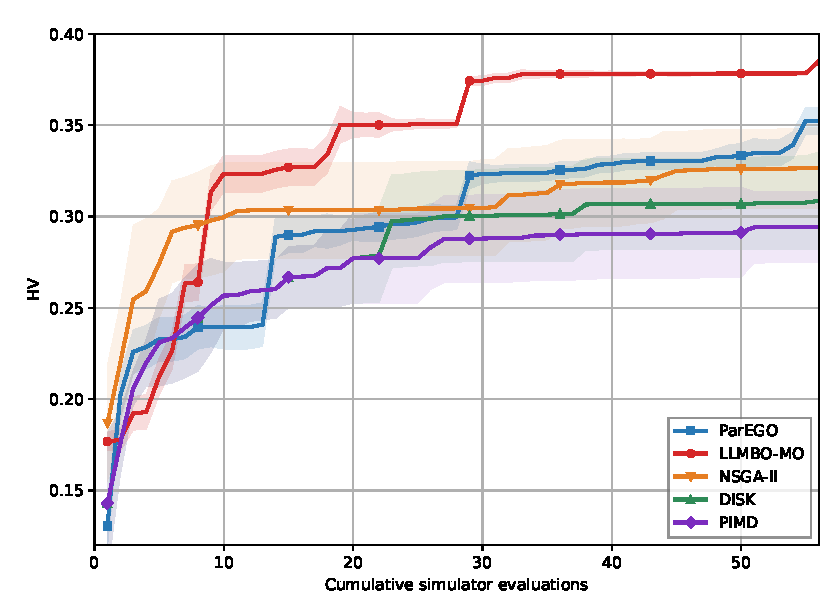
\includegraphics[width=0.99\columnwidth]{chen2020_hv_5way.pdf}
\caption{HV trajectories of the five methods on Chen2020.}
\label{fig:chen_hv_5way}
\end{figure}

\begin{table}[!t]
\caption{Final HV on Chen2020}
\label{tab:chen_results}
\centering
\footnotesize
\setlength{\tabcolsep}{4.0pt}
\begin{tabular}{@{}lc@{}}
\toprule
Method & Final HV (mean $\pm$ SD) $\uparrow$ \\
\midrule
LLMBO-MO & \textbf{\ChenLLMBOMean\,$\pm$\,\ChenLLMBOStd} \\
ParEGO & \ChenParEGOMean\,$\pm$\,\ChenParEGOStd \\
NSGA-II & \ChenNSGAMean\,$\pm$\,\ChenNSGAStd \\
DISK & \ChenDISKMean\,$\pm$\,\ChenDISKStd \\
PIMD & \ChenPIMDMean\,$\pm$\,\ChenPIMDStd \\
\bottomrule
\end{tabular}
\end{table}

The comparison with ParEGO is repeated on Ecker2015. LLMBO-MO reaches
\EckerLLMBOMean\,$\pm$\,\EckerLLMBOStd\ at evaluation 56, whereas ParEGO
reaches \EckerParEGOMean\,$\pm$\,\EckerParEGOStd
(Table~\ref{tab:ecker_results}). Its HV is also higher over most of the search
in Fig.~\ref{fig:ecker_hv}. The advantage over ParEGO is therefore observed
with both battery parameterizations at the tested budget.

\begin{figure}[!t]
\centering
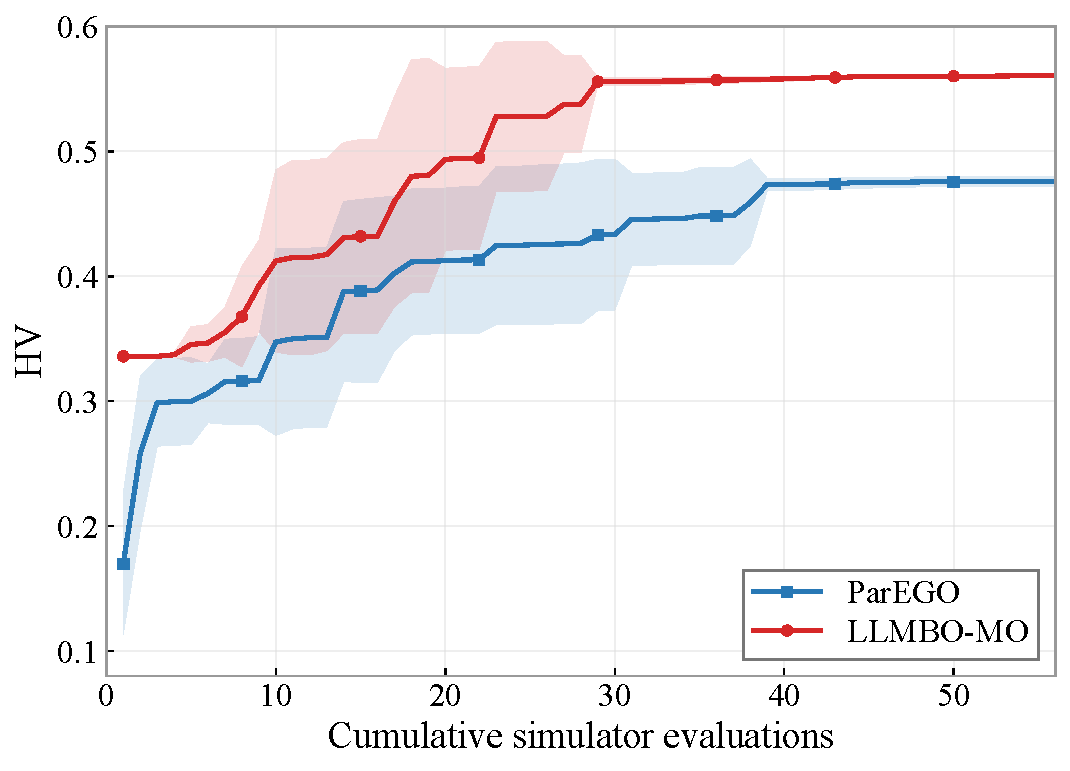
\includegraphics[width=0.99\columnwidth]{ecker2015_hv.pdf}
\caption{HV trajectories of LLMBO-MO and ParEGO on Ecker2015.}
\label{fig:ecker_hv}
\end{figure}

\begin{table}[!t]
\caption{HV Comparison on Ecker2015}
\label{tab:ecker_results}
\centering
\footnotesize
\setlength{\tabcolsep}{4.0pt}
\begin{tabular}{@{}lc@{}}
\toprule
Method & Evaluation 56 \\
\midrule
ParEGO & \EckerParEGOMean\,$\pm$\,\EckerParEGOStd \\
LLMBO-MO & \textbf{\EckerLLMBOMean\,$\pm$\,\EckerLLMBOStd} \\
\bottomrule
\end{tabular}
\end{table}

\subsection{Ablation Study}

The preceding comparisons assess the complete method. Two studies on
Chen2020 separate the effect of battery-specific prompting from the
contributions of initialization and regional guidance.

\subsubsection{LLM-Informed Initialization}

We compare random initialization, a detailed generic prompt, and a
battery-specific prompt (Figs.~\ref{fig:prompt_generic}
and~\ref{fig:prompt_warmstart}). All three variants use the same numerical BO
procedure after initialization. Each run has a budget of 26 evaluations,
and the results are computed over ten matched trials
(Table~\ref{tab:prompt_study}).

\begin{figure}[!t]
\centering
\promptbox{\footnotesize
You are an expert in lithium-ion battery fast-charging optimization. Task:
design $15$ diverse initial charging protocols for a multi-objective
Bayesian optimization workflow.\\
Decision variables and bounds: $I_1\in[2.0,6.0]$~A,
$I_2\in[2.0,5.0]$~A, $I_3\in[2.0,3.0]$~A,
$\Delta s_1\in[0.10,0.40]$, $\Delta s_2\in[0.10,0.30]$; hard constraint
$\Delta s_1+\Delta s_2<0.70$.\\
Objectives: minimize charging time, peak temperature rise, and capacity
fade.\\
Guidance: multi-objective optimization requires exploring different
trade-off directions (fast charging vs.\ thermal safety vs.\ aging
minimization); a good initial set should be well dispersed across the
five-dimensional decision space;
\textcolor{red!70!black}{consider leveraging physical relationships
between decision variables}; points near the boundary of the feasible
region can help maximize Pareto coverage, while interior points help model
the response surface in the central region. Respond with only a JSON
array.}
\caption{Generic prompt used in the initialization study of
Table~\ref{tab:prompt_study}. Unlike the battery-specific prompt in
Fig.~\ref{fig:prompt_warmstart}, it contains no battery-specific domain
knowledge.}
\label{fig:prompt_generic}
\end{figure}

\begin{table}[!t]
\caption{Effect of Different Initialization Strategies}
\label{tab:prompt_study}
\centering
\footnotesize
\setlength{\tabcolsep}{4.0pt}
\begin{tabular}{@{}lc@{}}
\toprule
Initialization & Final HV (mean $\pm$ SD) $\uparrow$ \\
\midrule
Random & 0.31062 $\pm$ 0.04303 \\
Generic prompt & 0.31371 $\pm$ 0.04675 \\
Battery-specific prompt & \textbf{0.36890 $\pm$ 0.00824} \\
\bottomrule
\end{tabular}
\end{table}

The generic prompt gives a mean final HV close to that of random
initialization: 0.31371 versus 0.31062. The battery-specific prompt reaches
0.36890, an increase of \PromptHVGain\ over random initialization, and has a
smaller standard deviation. The paired initialization analysis yields a
Holm-adjusted $p$-value of \PromptHolmP. The difference between generic and
battery-specific prompting indicates that the content of the domain
information matters for short-budget optimization, not merely the use of an
LLM to generate candidates.

\subsubsection{Regional Guidance}

Four variants are compared: the numerical BO optimizer without LLM guidance,
initialization only, regional guidance only, and the complete method. This
study uses three matched trials per variant. Each run contains six initial
evaluations followed by 50 BO iterations, giving a total budget of 56
battery-model evaluations. The results are summarized in
Table~\ref{tab:ablation} and Fig.~\ref{fig:ablation_hv_box}.

\begin{figure}[!t]

\centering

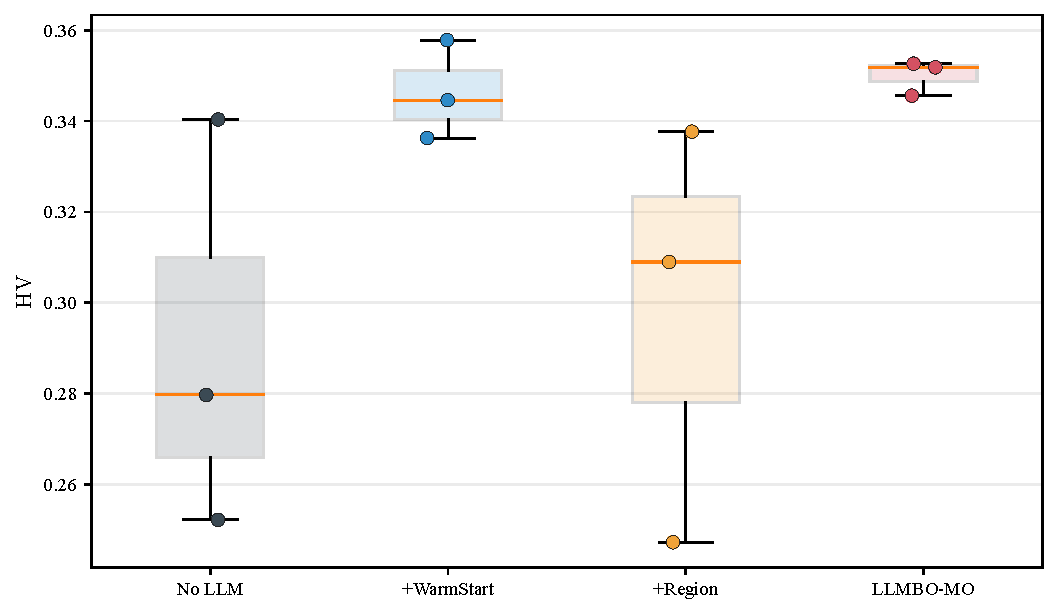
\includegraphics[width=0.99\columnwidth]{ablation_hv_box.pdf}

\caption{Final HV distributions of the four ablation variants on Chen2020.}

\label{fig:ablation_hv_box}

\end{figure}

\begin{table}[!t]

\caption{Ablation Results on Chen2020}

\label{tab:ablation}

\centering

\footnotesize

\setlength{\tabcolsep}{4.0pt}

\begin{tabular}{@{}lc@{}}

\toprule

Variant & Final HV (mean $\pm$ SD) $\uparrow$ \\

\midrule

No LLM & \AblationBaselineMean\,$\pm$\,\AblationBaselineStd \\

+ WarmStart & \AblationWarmMean\,$\pm$\,\AblationWarmStd \\

+ Regional guidance & \AblationRegionMean\,$\pm$\,\AblationRegionStd \\

LLMBO-MO & \textbf{\AblationFullMean\,$\pm$\,\AblationFullStd} \\

\bottomrule

\end{tabular}

\end{table}

Figure~\ref{fig:ablation_hv_box} and Table~\ref{tab:ablation} show that
LLM-informed initialization provides the largest improvement among the two
LLM-guidance components. Adding WarmStart increases the mean final HV from
\AblationBaselineMean\ to \AblationWarmMean, whereas regional guidance alone
reaches \AblationRegionMean. When regional guidance is added on top of
LLM-informed initialization, the mean final HV further increases from
\AblationWarmMean\ to \AblationFullMean. The complete method also has the
smallest sample standard deviation among the four variants.

The results indicate that the two components contribute at different stages
of the optimization. LLM-informed initialization improves the starting design
by directing the initial evaluations toward more promising charging protocols.
Region-Lift then uses the current scalarization weights to adjust candidate
selection during the subsequent BO iterations. In this comparison,
initialization provides most of the performance gain, while regional guidance
further improves the final optimization result.


\subsection{Comparison Across LLM Backends}

\label{sec:llm_backends}

To examine the effect of the LLM backend, Table~\ref{tab:llm_backends}
compares three models using the same Chen2020 prompt, numerical BO settings,
and evaluation budget. Each backend is evaluated in a single run consisting
of six initial evaluations followed by 50 BO iterations, for a total of 56
battery-model evaluations.

\begin{table}[!t]

\caption{HV Obtained with Different LLM Backends}

\label{tab:llm_backends}

\centering

\footnotesize

\setlength{\tabcolsep}{4.5pt}

\begin{tabular}{@{}lccc@{}}

\toprule

Backend & Initial HV & HV at 15 & Final HV \\

\midrule

DeepSeek-V4-Flash & 0.341225 & \textbf{0.373845} & 0.385986 \\

DeepSeek-V4-Pro & 0.345274 & 0.372526 & \textbf{0.387931} \\

GLM-5.3-Flash & \textbf{0.346248} & 0.372527 & 0.385324 \\

\bottomrule

\end{tabular}

\end{table}

The three backends produce different initial HV values, ranging from
0.341225 to 0.346248, indicating that the initial protocols generated by
the LLM depend to some extent on the backend. As the BO search proceeds,
however, the difference becomes smaller. At evaluation 15, the HV values
are concentrated between 0.372526 and 0.373845. After the full evaluation
budget, the final HV values are 0.385986, 0.387931, and 0.385324 for
DeepSeek-V4-Flash, DeepSeek-V4-Pro, and GLM-5.3-Flash, respectively.

Although the three LLMs produce somewhat different initial designs, their
optimization trajectories become closer after subsequent BO updates and
lead to similar final HV values. This suggests that the LLM backend mainly
affects the initial proposals, while the numerical BO procedure reduces
these differences as additional battery-model evaluations are collected.

\subsection{Analysis of Pareto-Optimal Charging Protocols}

HV evaluates the nondominated set as a whole. To examine the charging choices
represented by that set, we select protocols A--C from the Chen2020 Pareto
archive. Figure~\ref{fig:pareto_profiles} shows their objective values, and
Table~\ref{tab:representative_protocols} gives their currents and SOC
increments.

\begin{figure}[!t]
\centering
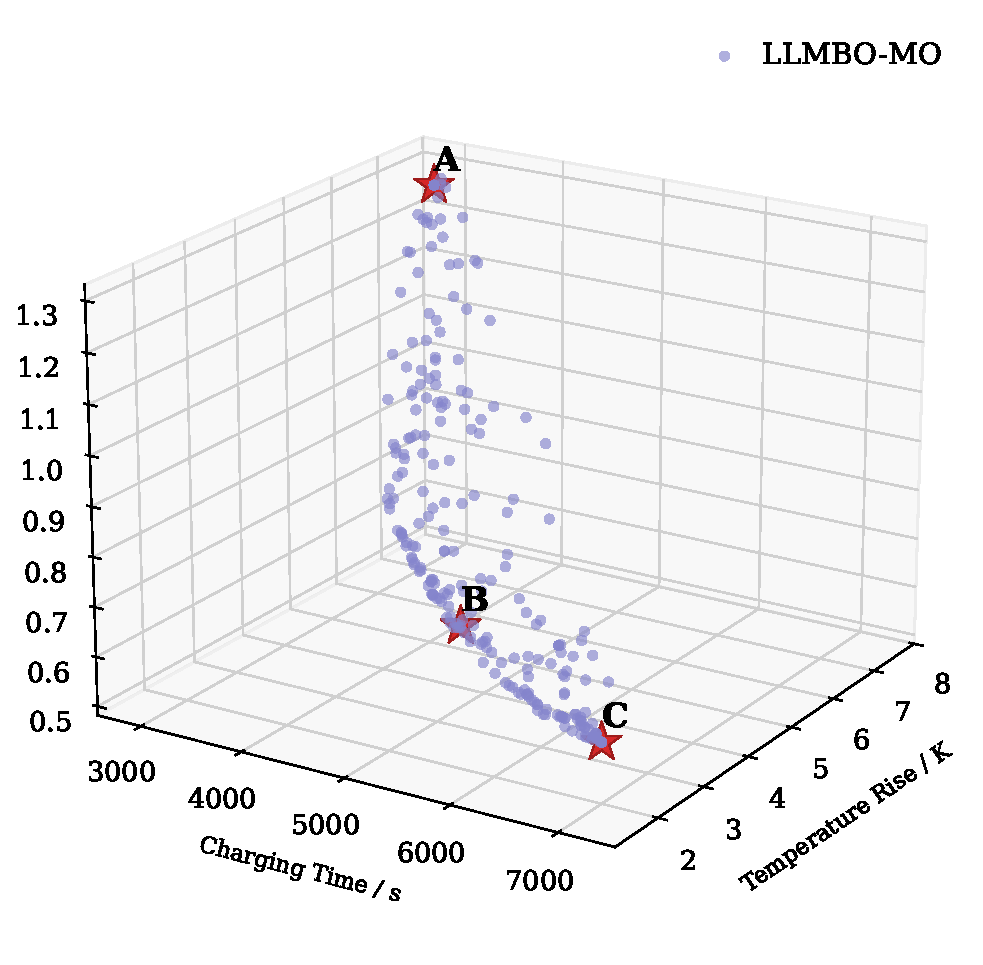
\includegraphics[width=\columnwidth]{pareto_protocols_ae.pdf}
\caption{Representative Pareto-optimal charging protocols on Chen2020.}
\label{fig:pareto_profiles}
\end{figure}

\begin{table*}[!t]
\caption{Representative Pareto-Optimal Charging Protocols}
\label{tab:representative_protocols}
\centering
\footnotesize
\setlength{\tabcolsep}{5.0pt}
\begin{tabular}{@{}c l r r r@{}}
\toprule
Protocol & $I_1/I_2/I_3/\Delta s_1/\Delta s_2/\Delta s_3$ &
$t_c$ (s) & $T_p$ (K) & $Q_s$ \\
\midrule
A & 6.000/5.000/3.000/0.400/0.300/0.100 & 2880 & 7.567 & 1.261 \\
B & 2.782/2.000/3.000/0.211/0.100/0.489 & 5199 & 3.069 & 0.680 \\
C & 2.000/2.000/2.000/0.245/0.153/0.403 & 7200 & 1.528 & 0.640 \\
\bottomrule
\end{tabular}
\end{table*}

Protocol A applies higher currents early in charging and reaches the target
SOC in 2880~s. It is the fastest of the three, but has the largest peak
temperature rise and aging indicator. Protocol C uses a constant 2~A current
and takes 7200~s, with the lowest values of both indicators. Protocol B offers
an intermediate choice: relative to C, it reduces charging time to 5199~s,
while the aging indicator increases from 0.640 to 0.680 and peak temperature
rise from 1.528 to 3.069~K. The benefit of faster charging can thus be weighed
against its thermal and degradation costs using the returned protocols.

Figure~\ref{fig:abc_charging_profiles} shows the voltage, temperature,
current, and SOC trajectories. The current transitions distinguish the
multistage protocols A and B from the constant-current protocol C, and the SOC
curves show their different completion times. The voltage trajectories remain
below the prescribed limit.

\begin{figure}[!t]
\centering
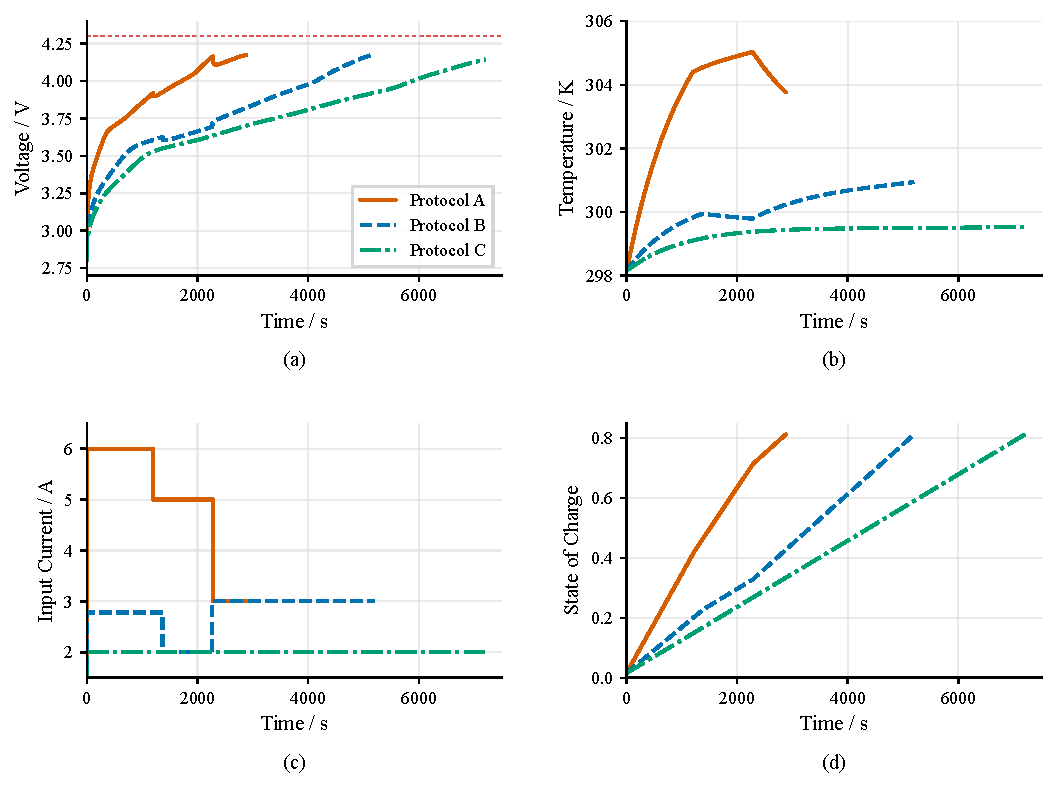
\includegraphics[width=\columnwidth]{abc_charging_profiles.pdf}
\caption{Charging trajectories of protocols A--C on Chen2020.}
\label{fig:abc_charging_profiles}
\end{figure}

\section{Conclusion}
\label{sec:conclusion}

LLMBO-MO incorporates battery-domain knowledge into multiobjective charging
optimization through initial protocol proposals and regional preferences for
successive scalarized subproblems. The Region-Lift adaptation uses GP
posterior cross-covariance to translate the regional preferences into mean
adjustments when computing EI.

With 56 battery-model evaluations, LLMBO-MO achieved a mean final HV of
\ChenLLMBOMean\ on Chen2020, compared with \ChenParEGOMean\ for ParEGO,
a \ChenFinalGain\ increase. The corresponding Ecker2015 values were
\EckerLLMBOMean\ and \EckerParEGOMean. In the 16-evaluation component study,
initialization accounted for most of the improvement, while adding regional
guidance increased the mean HV from \AblationWarmMean\ to \AblationFullMean.
The initialization study further showed that battery-specific prompting
improved short-budget optimization more than generic prompting. These findings
support the use of qualitative battery knowledge to improve the early search
for charging trade-offs. Future work will assess regional guidance over wider
operating conditions and validate the resulting protocols on physical cells
with measured degradation.

% ============================================================================
% Appendices: optional mechanism and supporting diagnostics
% ============================================================================
\appendices

\section{Optional Bounded Preference Coupling}
\label{app:coupling}

Accepted regional anchors can additionally be translated into a bounded
adjustment of the acquisition mean.
This posterior-mean coupling is a diagnostic variant that is separate from the
acquisition-restart regional guidance used by the principal LLMBO-MO
configuration; it is therefore analyzed independently here.

Let $\bG_t=\{\mathbf g_{j,t}\}_{j=1}^{M}$ denote accepted anchors.
Each anchor is scored using its EI value, posterior uncertainty, and novelty:
\begin{equation}
\begin{aligned}
n_{j,t}
&=\min_{\mathbf x\in\bD_t}
\|\widehat{\mathbf g}_{j,t}-\widehat{\mathbf x}\|_2,\\
s_{j,t}
&=\eta_{\mathrm{EI}}z\!\left(
\log\max\{\mathrm{EI}_{j,t},\varepsilon_{\mathrm{EI}}\}\right)
+\eta_\sigma z(\sigma_{j,t})+\eta_n z(n_{j,t}),\\
v_{j,t}
&=\frac{\exp(s_{j,t}/T_v)}
{\sum_{\ell=1}^{M}\exp(s_{\ell,t}/T_v)}.
\end{aligned}
\label{eq:anchor_weights}
\end{equation}
If anchor scoring is unavailable numerically, uniform weights
$v_{j,t}=1/M$ are used.

Let $\boldsymbol\Sigma_{GG,t}$ be the posterior covariance among anchors and
$\boldsymbol\Sigma_{\theta G,t}$ the candidate-to-anchor covariance.
The posterior correlation between a candidate and the weighted anchor portfolio
is
\begin{equation}
\begin{aligned}
V_{G,t}
&=\mathbf v_t^\top
(\boldsymbol\Sigma_{GG,t}+\varepsilon_K\mathbf I)\mathbf v_t,\\
\rho_t(\btheta)
&=\frac{\boldsymbol\Sigma_{\theta G,t}\mathbf v_t}
{\sigma_t(\btheta)\sqrt{\max\{V_{G,t},\varepsilon_v\}}}.
\end{aligned}
\label{eq:covariance_projection}
\end{equation}
Only positive correlations are used to attract EI toward preferred regions.

The region-quality gate combines the concentration of anchor weights and the
dispersion of anchor scores:
\begin{equation}
\begin{aligned}
H_t&=-\sum_{j=1}^{M}v_{j,t}\log(v_{j,t}+\varepsilon_H),\\
\bar H_t&=\frac{H_t}{\max\{\log M,\varepsilon_H\}},\\
q_t&=\operatorname{clip}\!\left[
\eta_H(1-\bar H_t)
+(1-\eta_H)\tanh\!\bigl(\operatorname{std}(\mathbf s_t)\bigr),
0,1\right].
\end{aligned}
\label{eq:quality_gate}
\end{equation}
The LLM-reported confidence
$c_t=\operatorname{clip}(h_t^{\mathrm{LLM}},0,1)$ and a bounded trust factor
$\tau_t\in[0,1]$ define $r_t=c_t\tau_tq_t$.
The attenuation $a_t=\operatorname{clip}(1-(t-1)/T_{\mathrm L},0,1)$ reduces
the possible influence to zero by the end of the guidance window.
The bounded adjustment is
\begin{equation}
\begin{aligned}
\delta_t(\btheta)
&=\operatorname{clip}\!\left(
a_t\lambda_{\max}r_t[\rho_t(\btheta)]_+,
0,\delta_{\max}\right),\\
\mu_t^{\mathrm L}(\btheta)
&=\mu_t(\btheta)-\delta_t(\btheta),\\
(\sigma_t^{\mathrm L})^2(\btheta)&=\sigma_t^2(\btheta).
\end{aligned}
\label{eq:bounded_coupling}
\end{equation}
Because \eqref{eq:tchebycheff} is minimized, decreasing the posterior mean near
positively correlated anchors increases their attractiveness to EI.
Clipping limits the adjustment in standardized scalar-target units, preserves
the posterior variance, and creates no pseudo-observation.
The principal results use regional information only as acquisition-search
restarts and therefore do not rely on \eqref{eq:bounded_coupling}.

\section{Supporting Numerical Diagnostics}
\label{app:diagnostics}

\subsection{Pareto-Archive Growth}

The archive-growth diagnostic tracks the number of feasible
Pareto-nondominated protocols retained during optimization.
It describes archive richness and is not used as a substitute for HV or as a
primary sample-efficiency metric.
Here, an ``optimal charging protocol'' means a feasible Pareto-nondominated
entry in the current archive.

\begin{figure}[H]
\centering
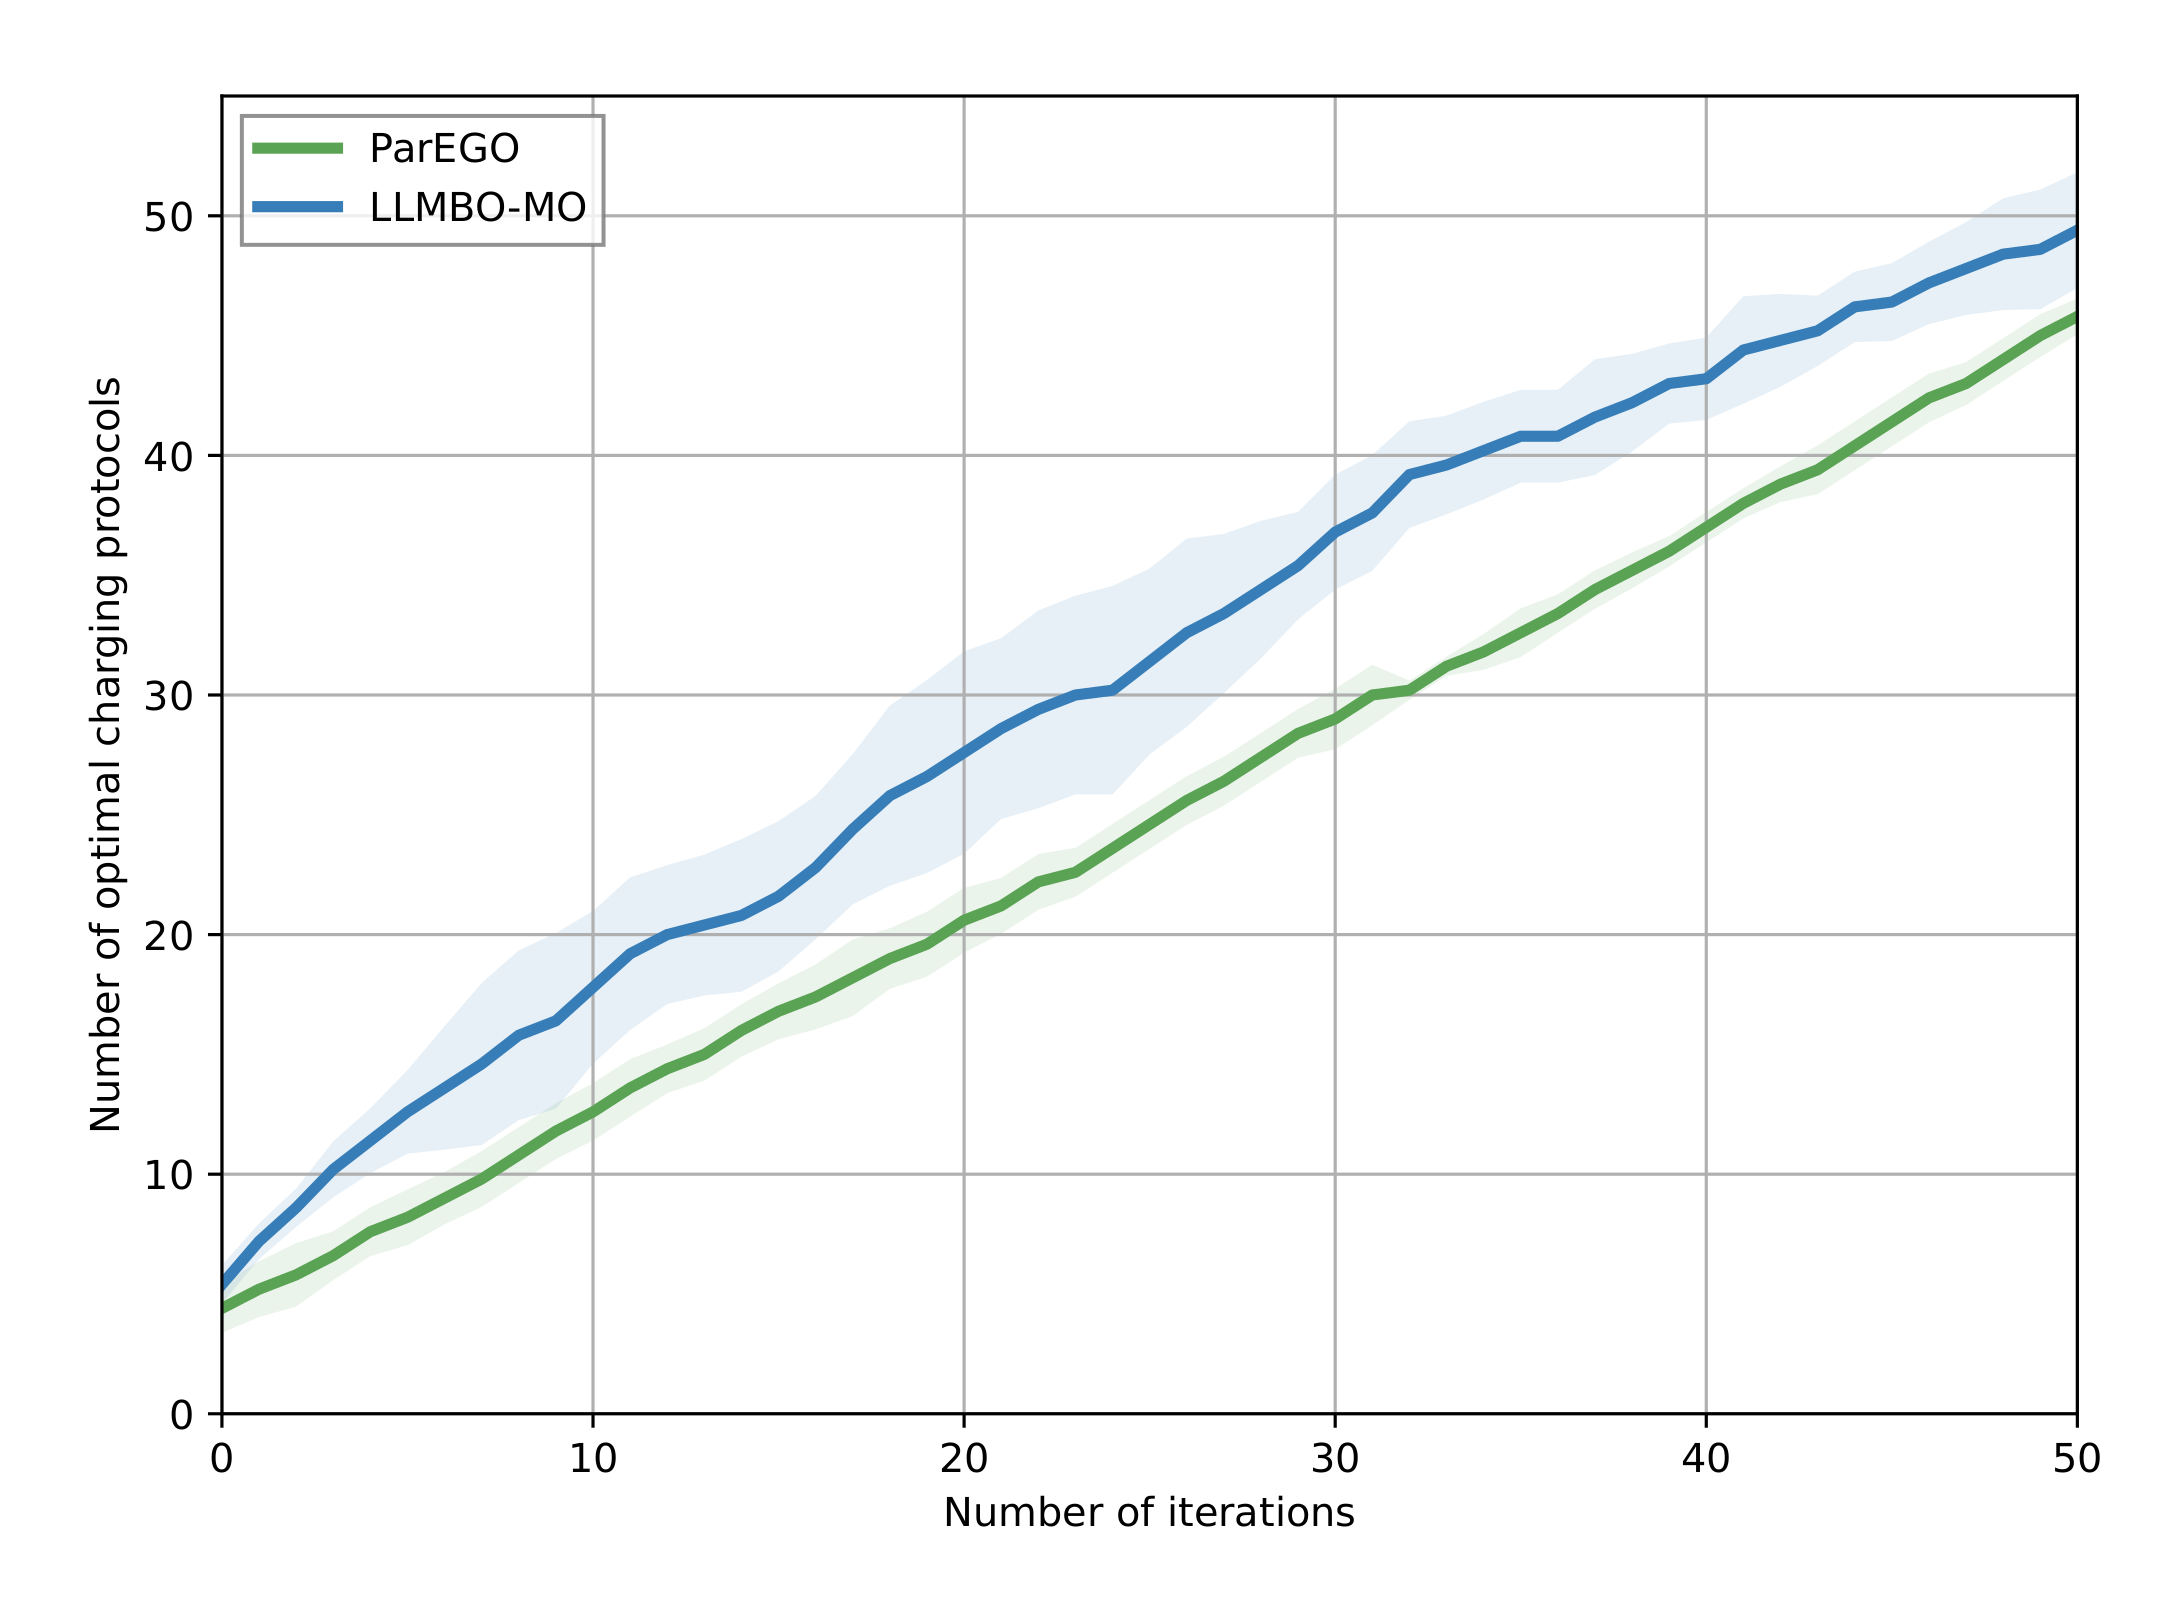
\includegraphics[width=0.99\columnwidth]{optimal_protocols_curve_600dpi.png}
\caption{Chen2020 Pareto-archive growth over 50 algorithmic iterations. Lines
are five-seed means and bands show across-seed dispersion.}
\label{fig:optimal_protocols}
\end{figure}

At iteration 50, LLMBO-MO maintains an average of approximately
\OptimalLLMBOFinal\ nondominated protocols, compared with
\OptimalParEGOFinal\ for ParEGO.
Its curve remains higher through most of the search, indicating a richer
retained set of trade-offs across these seeds.
Because the horizontal axis counts algorithmic iterations,
Fig.~\ref{fig:optimal_protocols} is not an equal-simulator-call sample-efficiency
comparison and is independent of the fixed-budget HV result.

\subsection{Objective-Scaling Sensitivity}

The scaling diagnostic compares min--max scaling, Z-score standardization, and
no normalization on Chen2020 over five seeds and the same 56-evaluation budget.
It tests numerical robustness rather than the LLM mechanism.

\begin{figure}[H]
\centering
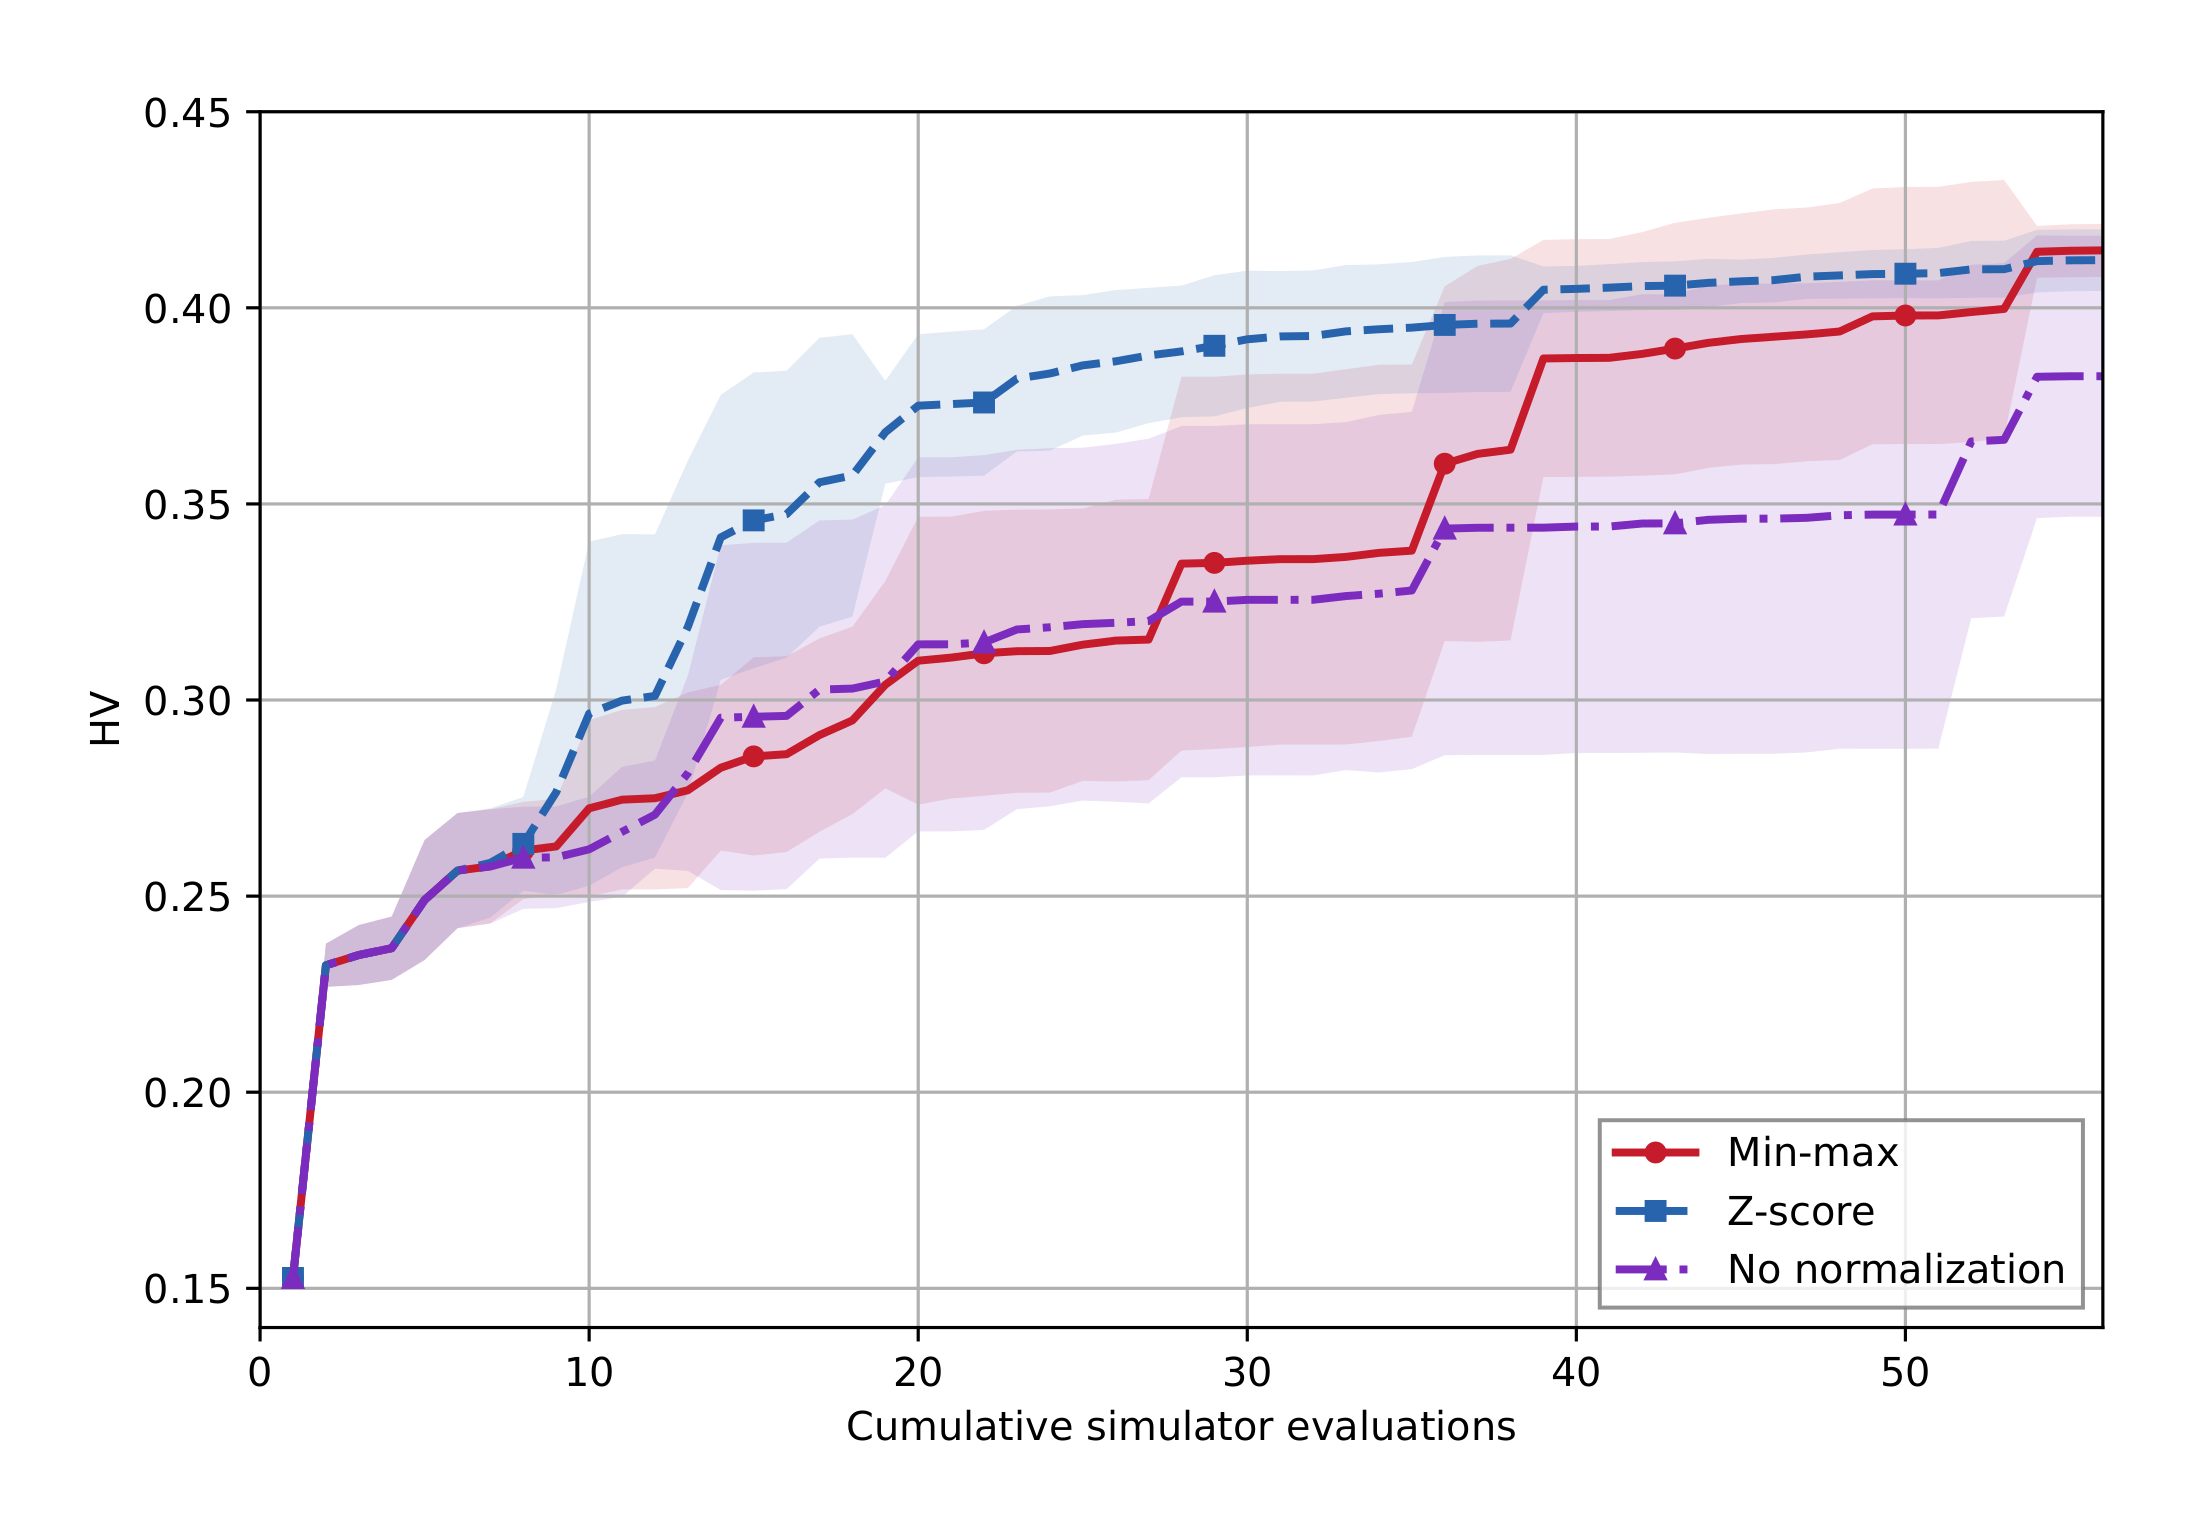
\includegraphics[width=0.99\columnwidth]{objective_normalization_hv_600dpi.png}
\caption{Chen2020 objective-preprocessing sensitivity over five seeds. Lines
show mean HV and bands show one sample standard deviation.}
\label{fig:normalization_hv}
\end{figure}

\begin{table}[!t]
\caption{Objective-Preprocessing Sensitivity on Chen2020}
\label{tab:normalization_hv}
\centering
\footnotesize
\setlength{\tabcolsep}{3.8pt}
\begin{tabular}{@{}lcc@{}}
\toprule
Preprocessing & Evaluation 30 & Evaluation 56 \\
\midrule
Min--max & \NormMidMinMax & \NormMinMaxMean\,$\pm$\,\NormMinMaxStd \\
Z-score & \textbf{\NormMidZScore} & \NormZScoreMean\,$\pm$\,\NormZScoreStd \\
None & \NormMidNone & \NormNoneMean\,$\pm$\,\NormNoneStd \\
\bottomrule
\end{tabular}
\end{table}

Z-score preprocessing progresses faster in the middle of the search, reaching
an HV of \NormMidZScore\ at evaluation 30 compared with \NormMidMinMax\ for
min--max scaling.
At evaluation 56, min--max scaling has the slightly higher mean
(\NormMinMaxMean\ versus \NormZScoreMean), but the difference is small and is
not interpreted as a significant ordering.
Both scale-balancing choices have substantially lower final dispersion than
the unnormalized condition, whose final result is
\NormNoneMean\,$\pm$\,\NormNoneStd.
Thus, heterogeneous objective magnitudes should be balanced, while either
conventional scaling choice is defensible in the present setting.


\section{Seed Configuration and Reproducibility}
\label{app:reproducibility}

The main Chen2020 and Ecker2015 comparisons use the same five seeds
(\MainSeedSet) for each method.
The reported studies share a common configuration:

\begin{itemize}
\item Chen2020 main comparison: five seeds (\MainSeedSet);
56 simulator calls per seed.
\item Ecker2015 second-parameterization case: five seeds
(\MainSeedSet); 56 simulator calls per seed.
\item Initialization study: ten matched seeds; 26-call budget.
\item Component ablation: three matched seeds (8409--8411);
16-call budget.
\item Main regional guidance: $T_{\mathrm L}=16$, 64 anchors,
EI-search restarts.
\item LLM records: prompt configuration and responses logged per
seed.
\end{itemize}

Seed-level identifiers, LLM call records, and parsed responses are
retained in the experiment logs rather than in the main parameter
table so that the reported statistics can be traced to the
corresponding seed set without interrupting the main experimental
narrative.

For the main algorithm, regional information affects only
acquisition-search restarts. The posterior-mean coupling in
Appendix~\ref{app:coupling} is a separate diagnostic realization and
is not used to define the principal results.

% ============================================================================
% References (hand-written thebibliography; no external .bib needed)
% ============================================================================
\begin{thebibliography}{14}

\bibitem{ref1}
N.~Nitta \textit{et al.}, ``Li-ion battery materials: present and future,''
\textit{Materials Today}, vol.~18, no.~5, pp.~252--264, 2015.

\bibitem{ref2}
A.~Tomaszewska \textit{et al.}, ``Lithium-ion battery fast charging: A review,''
\textit{eTransportation}, vol.~1, p.~100011, 2019.

\bibitem{ref3}
B.~Shahriari \textit{et al.}, ``Taking the human out of the loop: A review of
Bayesian optimization,'' \textit{Proc. IEEE}, vol.~104, no.~1, pp.~148--175,
2016.

\bibitem{ref4}
J.~Knowles, ``ParEGO: A hybrid algorithm with on-line landscape approximation
for expensive multiobjective optimization problems,'' \textit{IEEE Trans. Evol.
Comput.}, vol.~10, no.~1, pp.~50--66, 2006.

\bibitem{ref5}
K.~Deb \textit{et al.}, ``A fast and elitist multiobjective genetic algorithm:
NSGA-II,'' \textit{IEEE Trans. Evol. Comput.}, vol.~6, no.~2, pp.~182--197,
2002.

\bibitem{ref6}
S.~G.~Marquis \textit{et al.}, ``An asymptotic derivation of a single particle
model with electrolyte,'' \textit{J. Electrochem. Soc.}, vol.~166, no.~15,
pp.~A3693--A3706, 2019.

\bibitem{ref7}
V.~Sulzer \textit{et al.}, ``Python Battery Mathematical Modelling (PyBaMM),''
\textit{J. Open Res. Softw.}, vol.~9, no.~1, p.~14, 2021.

\bibitem{ref8}
C.~H.~Chen \textit{et al.}, ``Development of experimental techniques for
parameterization of multi-scale lithium-ion battery models,''
\textit{J. Electrochem. Soc.}, vol.~167, no.~8, p.~080534, 2020.

\bibitem{ref9}
M.~Ecker \textit{et al.}, ``Parameterization of a physico-chemical model of a
lithium-ion battery: I. Determination of parameters from electrochemical
impedance spectroscopy,'' \textit{J. Power Sources}, vol.~295, pp.~145--154,
2015.

\bibitem{ref10}
T.~Brown \textit{et al.}, ``Language models are few-shot learners,'' in
\textit{Advances in Neural Information Processing Systems}, vol.~33, 2020.

\bibitem{ref11}
X.~Li \textit{et al.}, ``Data-driven multi-objective optimization for battery
charging,'' \textit{IEEE Trans. Intell. Veh.}, vol.~8, no.~3,
pp.~2456--2467, 2023.

\bibitem{ref12}
Y.~Zhang \textit{et al.}, ``Physics-informed model-driven optimization for fast
charging protocol design,'' \textit{Appl. Energy}, vol.~335, p.~120728, 2023.

\bibitem{ref13}
J.~Jiang \textit{et al.}, ``Bayesian optimization for charging protocol
design,'' \textit{IEEE Trans. Ind. Electron.}, vol.~71, no.~4,
pp.~4120--4131, 2024.

\bibitem{ref14}
S.~Krishnamoorthy \textit{et al.}, ``Large language models for automated design
optimization,'' \textit{arXiv preprint arXiv:2402.06196}, 2024.

\end{thebibliography}


\end{document}
